\chapter{Pola Struktural 2}

Pola struktural lanjutan meliputi pola yang membantu menyederhanakan struktur antar objek dan memfasilitasi komunikasi yang efisien dalam sistem yang kompleks. Bab ini mencakup pola \textit{Facade}, \textit{Proxy}, dan \textit{Flyweight}.

\section{Facade}

\subsection{Tujuan dan Konteks Penggunaan}

Pola \textit{Facade} adalah salah satu pola struktural yang dirancang untuk menyediakan antarmuka tunggal yang menyederhanakan akses ke subsistem atau kumpulan kelas yang kompleks. Dalam sistem perangkat lunak yang besar, seringkali terdapat berbagai komponen atau modul yang saling berinteraksi, masing-masing dengan antarmuka yang kompleks dan ketergantungan yang erat. Pola \textit{Facade} bertujuan untuk menyembunyikan kompleksitas internal ini dengan memberikan pintu masuk (interface) tunggal yang mudah digunakan oleh klien.

\textbf{Tujuan utama dari pola Facade adalah:}
\begin{itemize}
	\item Menyederhanakan penggunaan subsistem yang kompleks dengan menyediakan antarmuka tingkat tinggi.
	\item Mengurangi ketergantungan langsung antara klien dan komponen internal sistem.
	\item Meningkatkan pemisahan tanggung jawab antara bagian sistem yang berbeda.
\end{itemize}

Pola ini sangat berguna dalam situasi berikut:
\begin{itemize}
	\item Ketika klien hanya membutuhkan subset dari fungsi subsistem yang kompleks.
	\item Saat ingin menyederhanakan proses integrasi antara subsistem dan modul eksternal.
	\item Untuk meningkatkan maintainability sistem dengan membatasi titik masuk ke komponen internal.
\end{itemize}

\textbf{Analogi dunia nyata:} Seperti halnya resepsionis di hotel yang bertindak sebagai titik kontak tunggal bagi tamu untuk mendapatkan layanan seperti pemesanan kamar, layanan kamar, dan informasi lokal—pola \textit{Facade} menyediakan satu antarmuka terpadu yang menyederhanakan akses ke berbagai layanan internal dalam sistem.

Dengan menerapkan pola \textit{Facade}, sistem menjadi lebih modular dan fleksibel. Klien tidak perlu mengetahui detail teknis atau urutan pemanggilan dari berbagai komponen yang terlibat. Ini menjadikan kode lebih bersih, lebih mudah diuji, dan lebih mudah untuk diubah atau diperluas.

\subsection{Contoh Kasus Penggunaan}

Pola \textit{Facade} sangat efektif digunakan ketika sistem memiliki banyak subsistem atau modul dengan antarmuka yang kompleks, dan pengguna (klien) hanya membutuhkan operasi-operasi umum tanpa harus memahami detail internal setiap subsistem.

\textbf{Contoh 1: Sistem Pemesanan Tiket Online}

Dalam sebuah aplikasi pemesanan tiket (kereta, pesawat, konser), terdapat berbagai komponen seperti:
\begin{itemize}
	\item \texttt{UserAccountService} untuk autentikasi pengguna.
	\item \texttt{PaymentService} untuk memproses pembayaran.
	\item \texttt{SeatReservationService} untuk pemesanan kursi.
	\item \texttt{NotificationService} untuk mengirim email konfirmasi.
\end{itemize}

Tanpa \textit{facade}, klien perlu memanggil setiap layanan ini secara langsung dan menangani urutan serta dependensinya. Dengan menerapkan \texttt{BookingFacade}, klien cukup memanggil satu metode seperti \texttt{bookTicket()}, dan facade akan mengatur seluruh proses di balik layar secara terkoordinasi.

\textbf{Contoh 2: Kompilasi Kode dalam IDE}

IDE seperti IntelliJ atau Eclipse memiliki subsistem untuk:
\begin{itemize}
	\item Parsing dan analisis sintaks.
	\item Pemeriksaan semantik dan referensi simbol.
	\item Optimisasi kode.
	\item Proses kompilasi dan link.
\end{itemize}

Daripada meminta pengguna untuk menjalankan setiap langkah secara manual, IDE menyediakan tombol “Compile” yang bertindak sebagai facade—menyederhanakan proses kompleks menjadi satu aksi yang intuitif.

\textbf{Contoh 3: Pembuatan Laporan Keuangan}

Sistem ERP yang menghasilkan laporan keuangan biasanya perlu menarik data dari berbagai modul:
\begin{itemize}
	\item Modul inventori.
	\item Modul transaksi penjualan dan pembelian.
	\item Modul akuntansi.
\end{itemize}

\texttt{ReportFacade} dapat mengoordinasikan pengambilan data, pemrosesan, dan penggabungan hasil menjadi satu laporan final, tanpa memaksa pengguna memahami cara masing-masing modul bekerja.

\textbf{Contoh Praktis Lain:}
\begin{itemize}
	\item \texttt{ComputerFacade} untuk menghidupkan komputer (menyalakan CPU, RAM, dan hard disk).
	\item \texttt{HomeTheaterFacade} untuk mengatur projector, audio system, dan layar dalam satu langkah.
	\item \texttt{StartupFacade} dalam arsitektur mikrosistem untuk menginisialisasi dependensi secara urut.
\end{itemize}

Dengan menggunakan pola \textit{Facade}, integrasi sistem menjadi lebih mudah dan penggunaan layanan kompleks menjadi lebih intuitif dan aman dari kesalahan urutan atau konfigurasi.


\subsection{Kelebihan dan Kekurangan}

Pola \textit{Facade} menawarkan berbagai keuntungan dalam menyederhanakan penggunaan sistem yang kompleks, namun seperti pola desain lainnya, terdapat juga beberapa keterbatasan yang perlu diperhatikan.

\textbf{Kelebihan:}
\begin{itemize}
	\item \textbf{Menyederhanakan antarmuka sistem:} Dengan menyediakan titik masuk tunggal, facade membuat sistem lebih mudah digunakan oleh klien yang tidak perlu mengetahui detail dari subsistem yang kompleks.
	
	\item \textbf{Meningkatkan keterpisahan (decoupling):} Klien tidak bergantung langsung pada detail internal subsistem, melainkan hanya pada facade. Ini meningkatkan fleksibilitas sistem dan memungkinkan perubahan di dalam subsistem tanpa memengaruhi kode klien.
	
	\item \textbf{Memfasilitasi standarisasi proses:} Facade dapat mengatur urutan pemanggilan dan validasi antara subsistem, sehingga memastikan bahwa proses selalu dijalankan dengan cara yang benar.
	
	\item \textbf{Mempermudah penggunaan sistem besar:} Dalam sistem yang terdiri dari banyak komponen dan antarmuka yang kompleks, facade membantu pengembang dan pengguna baru untuk berinteraksi dengan sistem tanpa perlu memahami setiap komponennya.
	
	\item \textbf{Cocok untuk integrasi layer-level:} Sangat berguna dalam konteks arsitektur berlapis seperti MVC atau mikrosistem, di mana facade dapat menyembunyikan kompleksitas layer bawah (seperti layanan domain atau database).
\end{itemize}

\textbf{Kekurangan:}
\begin{itemize}
	\item \textbf{Risiko abstractions yang terlalu sempit:} Jika tidak dirancang dengan baik, facade bisa terlalu menyederhanakan dan menyembunyikan fungsionalitas penting dari subsistem yang dibutuhkan oleh klien tertentu.
	
	\item \textbf{Potensi duplikasi logika:} Jika facade terlalu banyak meniru atau mengulangi logika yang sudah ada di subsistem, bisa terjadi redundansi dan sulit dipelihara.
	
	\item \textbf{Overhead tambahan:} Penerapan facade menambahkan lapisan baru dalam sistem. Meskipun tujuannya adalah untuk menyederhanakan, dalam beberapa kasus kecil atau sederhana, ini bisa menjadi beban arsitektur yang tidak perlu.
	
	\item \textbf{Peningkatan dependensi pada facade:} Jika semua akses hanya melalui facade, subsistem internal bisa menjadi tidak cukup diuji secara langsung, sehingga menyulitkan pengujian unit atau debugging.
	
	\item \textbf{Tidak mengurangi kompleksitas internal:} Facade hanya menyembunyikan kompleksitas, tetapi tidak menyederhanakan subsistem itu sendiri. Jika subsistem buruk, facade hanya menjadi penutup, bukan solusi.
\end{itemize}

Secara keseluruhan, pola \textit{Facade} ideal untuk sistem kompleks yang perlu diakses oleh banyak klien berbeda dengan kebutuhan yang umum. Namun, penerapannya harus disesuaikan dengan skala sistem dan tingkat fleksibilitas yang diinginkan.


\subsection{Implementasi dalam Java}

Implementasi pola \textit{Facade} dalam Java umumnya dilakukan dengan cara membuat sebuah kelas facade yang menjadi titik akses tunggal bagi klien untuk berinteraksi dengan sekumpulan subsistem yang kompleks. Kelas facade bertanggung jawab untuk menyatukan dan menyederhanakan pemanggilan metode dari berbagai kelas subsistem agar prosesnya lebih efisien dan mudah dipahami.

Secara umum, pola ini terdiri dari tiga komponen utama:
\begin{itemize}
	\item \textbf{Klien (Client):} Komponen yang membutuhkan layanan dari sistem yang kompleks, namun hanya berinteraksi dengan satu objek facade.
	\item \textbf{Facade:} Kelas yang menyediakan antarmuka tingkat tinggi dan menyederhanakan penggunaan subsistem.
	\item \textbf{Subsistem:} Sekelompok kelas atau layanan yang memiliki logika dan kompleksitas tersendiri, tetapi tersembunyi dari klien oleh facade.
\end{itemize}

Dalam implementasi Java, facade biasanya bersifat stateless, hanya berfungsi sebagai mediator atau koordinator. Namun dalam beberapa kasus, facade juga dapat menyimpan konfigurasi atau konteks yang diperlukan selama operasi.


\begin{figure}[h]
	\centering
	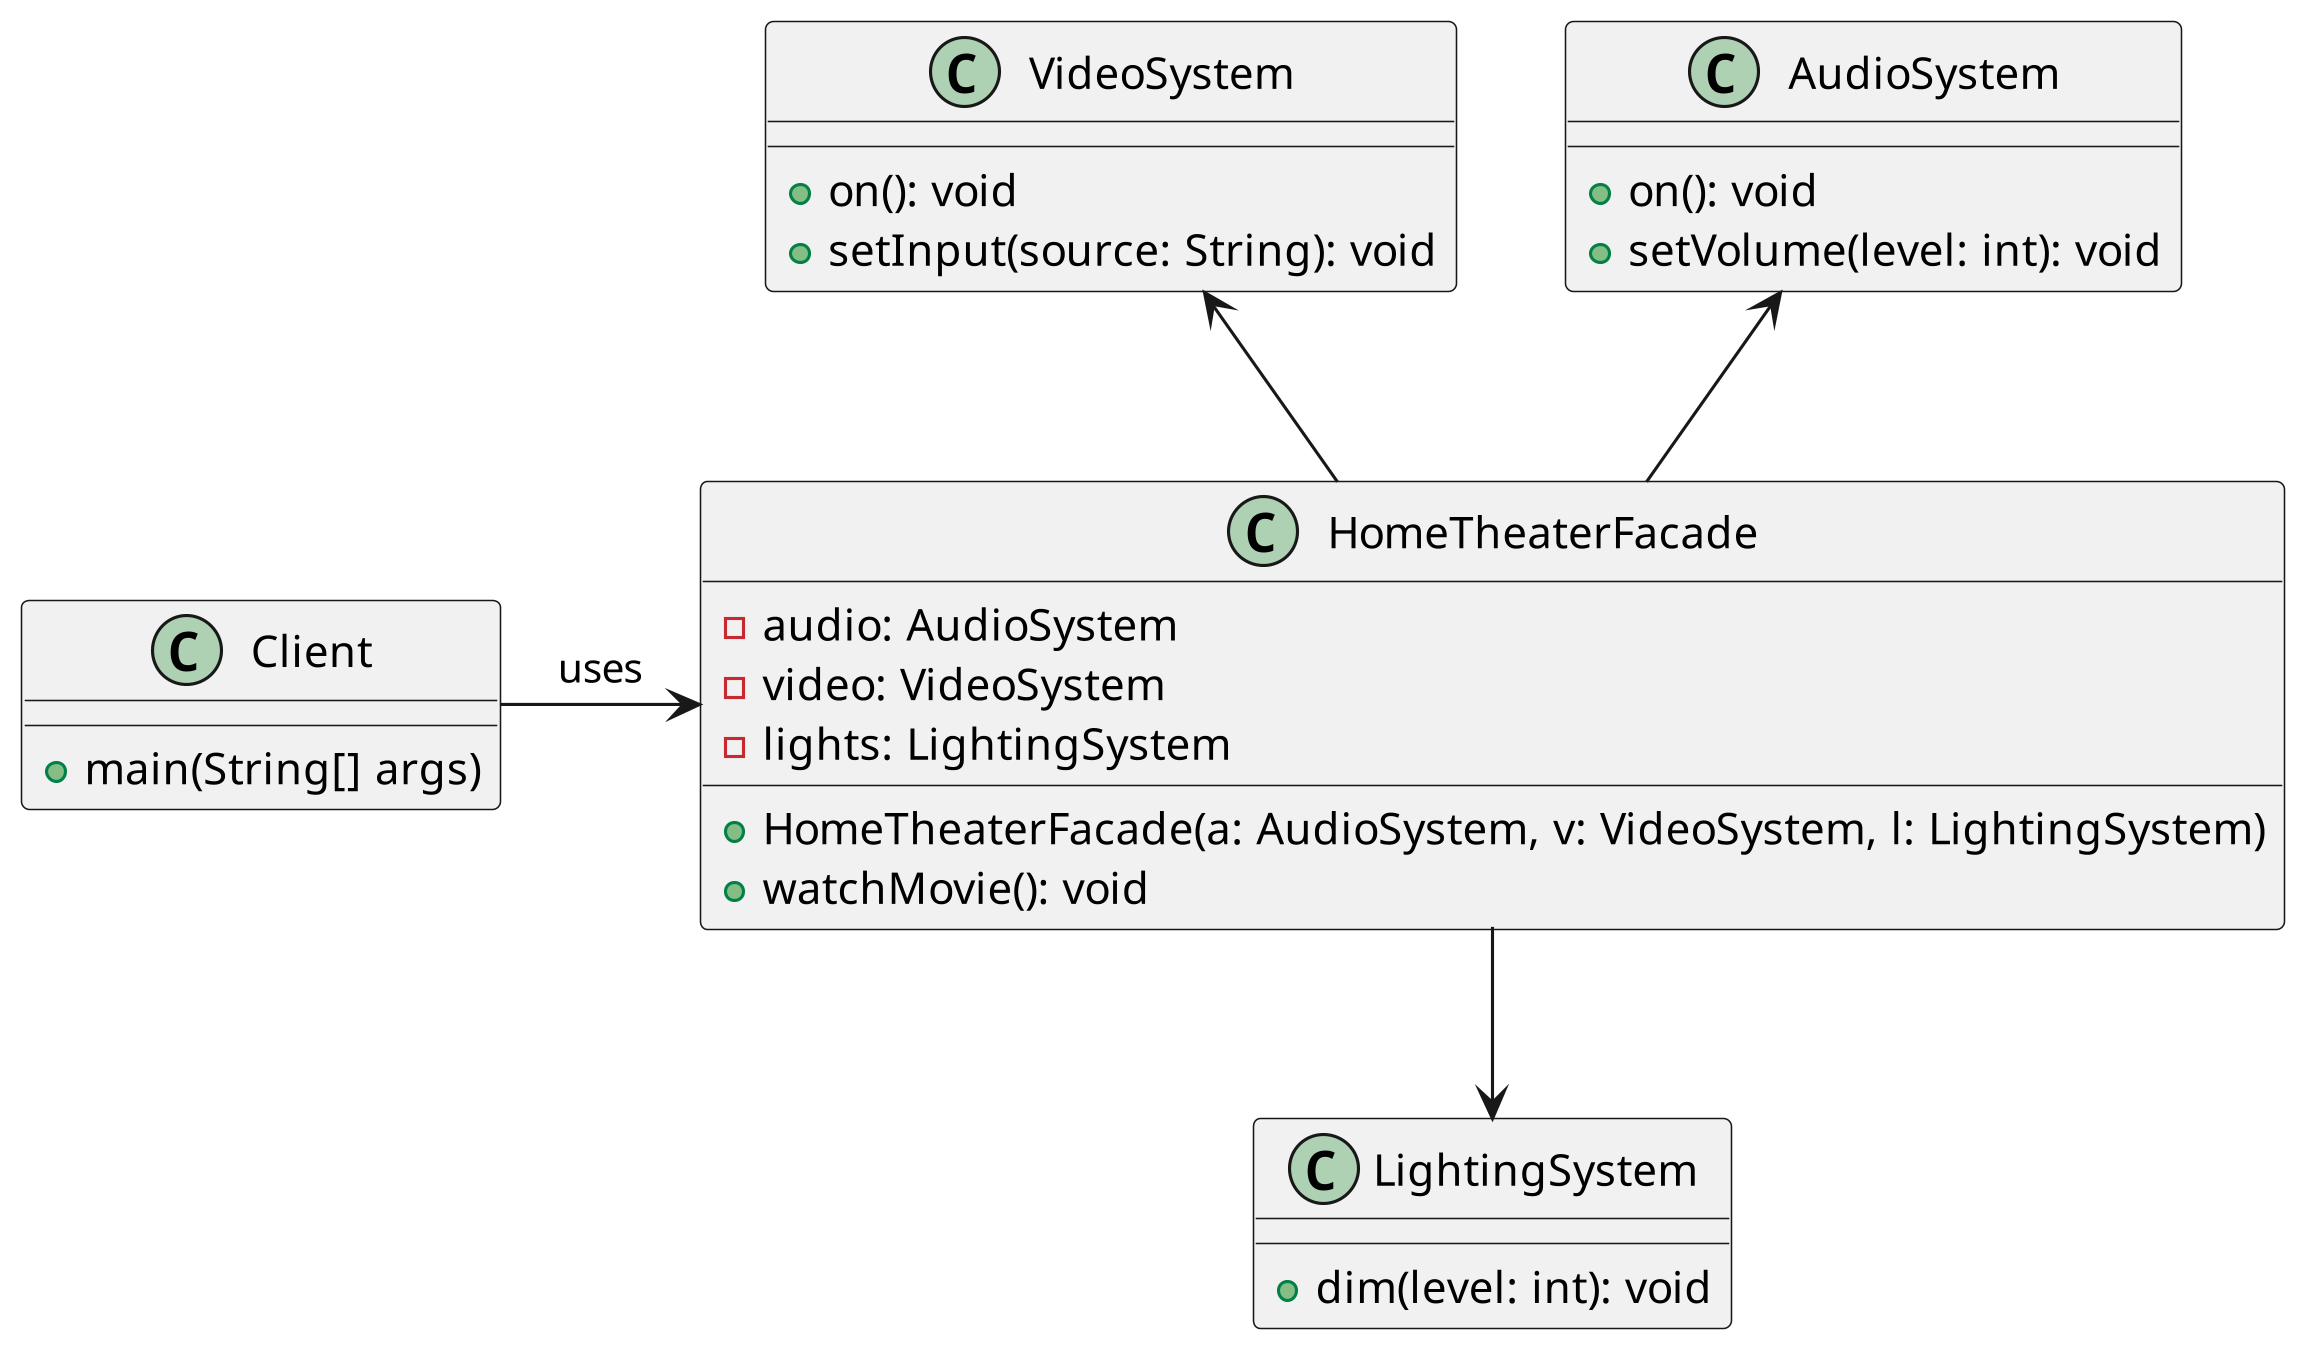
\includegraphics[width=\textwidth]{../figures/out/facade.png}
	\caption{Struktur Pola Facade}
	\label{fig:facade}
\end{figure}

Berikut adalah contoh sederhana untuk menggambarkan implementasi pola \textit{Facade} (Gambar \ref{fig:facade}). Dalam contoh ini, sistem terdiri dari tiga subsistem: \texttt{AudioSystem}, \texttt{VideoSystem}, dan \texttt{LightingSystem}, yang seluruhnya dikoordinasikan oleh kelas facade bernama \texttt{HomeTheaterFacade}.

\begin{lstlisting}[style=JavaStyle, caption={Subsistem: AudioSystem}]
	public class AudioSystem {
		public void on() {
			System.out.println("Audio system turned on.");
		}
		public void setVolume(int level) {
			System.out.println("Audio volume set to " + level);
		}
	}
\end{lstlisting}

\begin{lstlisting}[style=JavaStyle, caption={Subsistem: VideoSystem}]
	public class VideoSystem {
		public void on() {
			System.out.println("Video system turned on.");
		}
		public void setInput(String source) {
			System.out.println("Video input set to " + source);
		}
	}
\end{lstlisting}

\begin{lstlisting}[style=JavaStyle, caption={Subsistem: LightingSystem}]
	public class LightingSystem {
		public void dim(int level) {
			System.out.println("Lights dimmed to " + level + "%.");
		}
	}
\end{lstlisting}

\begin{lstlisting}[style=JavaStyle, caption={Facade: HomeTheaterFacade}]
	public class HomeTheaterFacade {
		private AudioSystem audio;
		private VideoSystem video;
		private LightingSystem lights;
		
		public HomeTheaterFacade(AudioSystem a, VideoSystem v, LightingSystem l) {
			this.audio = a;
			this.video = v;
			this.lights = l;
		}
		
		public void watchMovie() {
			lights.dim(30);
			audio.on();
			audio.setVolume(5);
			video.on();
			video.setInput("HDMI1");
			System.out.println("Movie is ready to play.");
		}
	}
\end{lstlisting}

\begin{lstlisting}[style=JavaStyle, caption={Client: Menggunakan Facade}]
	public class Main {
		public static void main(String[] args) {
			AudioSystem audio = new AudioSystem();
			VideoSystem video = new VideoSystem();
			LightingSystem lights = new LightingSystem();
			
			HomeTheaterFacade homeTheater = new HomeTheaterFacade(audio, video, lights);
			homeTheater.watchMovie();
		}
	}
\end{lstlisting}

Dalam contoh di atas, klien tidak perlu mengetahui detail cara menyalakan sistem audio, mengatur input video, atau meredupkan lampu. Semua proses ini telah dikemas dalam metode \texttt{watchMovie()} milik \texttt{HomeTheaterFacade}. Hal ini menjadikan kode klien jauh lebih bersih, mudah dibaca, dan tidak terikat pada perubahan yang mungkin terjadi pada subsistem internal.

Pola ini sangat berguna dalam pembangunan API, layanan mikro (microservices), sistem berlapis (layered architecture), dan sistem perangkat keras yang memiliki kontrol logika tersebar. Dengan menggunakan facade, kompleksitas dapat disembunyikan secara efektif tanpa mengorbankan fleksibilitas sistem.


\section{Proxy}

\subsection{Tujuan dan Konteks Penggunaan}

Pola \textit{Proxy} adalah salah satu pola desain struktural yang bertujuan untuk menyediakan objek pengganti atau perantara dari objek asli. Objek proxy mengontrol akses terhadap objek asli dengan cara menambahkan lapisan tambahan antara klien dan objek target. Pola ini sangat berguna ketika akses langsung ke objek sebenarnya tidak diinginkan atau tidak efisien karena alasan keamanan, performa, atau kendali.

Tujuan utama dari pola Proxy adalah:
\begin{itemize}
	\item Mengontrol akses ke objek yang memerlukan perlindungan atau kendali tambahan.
	\item Menunda inisialisasi objek yang berat hingga benar-benar diperlukan (lazy instantiation).
	\item Menyediakan fungsionalitas tambahan seperti logging, caching, autentikasi, atau remote access.
\end{itemize}

Secara umum, Proxy dapat menggantikan objek nyata dalam berbagai situasi tanpa mengubah antarmuka yang digunakan oleh klien. Ini berarti klien tidak perlu tahu apakah mereka berinteraksi dengan objek asli atau objek perantara.

Beberapa jenis proxy yang umum digunakan:
\begin{enumerate}
	\item \textbf{Virtual Proxy:} Digunakan untuk menunda pembuatan objek yang memakan sumber daya besar sampai benar-benar diperlukan. Contoh: memuat gambar besar atau database connection.
	\item \textbf{Protection Proxy:} Mengatur hak akses ke objek berdasarkan otorisasi pengguna. Contoh: akses file, antarmuka administratif.
	\item \textbf{Remote Proxy:} Mengelola komunikasi antara klien dan objek yang berada di lokasi fisik yang berbeda (misalnya jaringan). Contoh: RMI (Remote Method Invocation) atau Web Service.
	\item \textbf{Smart Proxy:} Menambahkan perilaku tambahan saat objek diakses, seperti logging, counting, atau validasi.
\end{enumerate}

Pola Proxy sering digunakan dalam pengembangan sistem skala besar, arsitektur berbasis layanan (SOA), pengelolaan sumber daya, serta dalam framework-framework modern seperti Spring dan Hibernate. Dengan menerapkan pola ini, pengembang dapat membangun sistem yang lebih aman, efisien, dan mudah dikelola tanpa mengganggu antarmuka pengguna atau logika bisnis utama.


\subsection{Contoh Kasus Penggunaan}

Pola \textit{Proxy} digunakan dalam berbagai situasi praktis di mana akses ke objek perlu dikendalikan, ditunda, atau dilindungi. Dalam dunia pengembangan perangkat lunak, pola ini memberikan fleksibilitas untuk menyisipkan logika tambahan di antara klien dan objek nyata tanpa memodifikasi kode klien atau objek tersebut secara langsung.

Berikut beberapa contoh kasus penggunaan nyata pola Proxy:

\textbf{1. Virtual Proxy: Menunda Pembuatan Objek Berat} \\
Dalam aplikasi pengolah dokumen atau editor gambar, objek seperti \texttt{LargeImage} mungkin memuat file gambar besar dari disk. Dengan menggunakan proxy, gambar tidak langsung dimuat ke memori saat dokumen dibuka, melainkan hanya saat gambar diperlukan untuk ditampilkan. Ini menghemat memori dan mempercepat waktu awal pemuatan dokumen.

\textbf{2. Protection Proxy: Kontrol Hak Akses} \\
Dalam aplikasi manajemen sistem, hanya pengguna tertentu yang boleh mengakses atau memodifikasi konfigurasi penting. Objek proxy dapat memverifikasi kredensial atau peran pengguna sebelum meneruskan permintaan ke objek asli. Contohnya, \texttt{AdminConfigProxy} membungkus \texttt{SystemConfig} dan hanya mengizinkan akses jika pengguna memiliki hak administratif.

\textbf{3. Remote Proxy: Akses Objek di Jaringan} \\
Dalam arsitektur terdistribusi seperti RMI (Remote Method Invocation) di Java atau REST API, objek proxy digunakan untuk mewakili objek yang berada di server jauh. Klien berinteraksi dengan proxy seolah-olah objek berada di memori lokal, namun proxy menangani komunikasi jaringan dan serialisasi data.

\textbf{4. Smart Proxy: Penambahan Fitur Tambahan} \\
Sebuah \texttt{SmartProxy} bisa digunakan untuk mencatat setiap kali suatu objek diakses, atau menghitung jumlah akses yang dilakukan. Misalnya, dalam aplikasi logistik, setiap kali data inventori dibaca atau dimodifikasi, proxy mencatat aktivitas tersebut untuk keperluan audit.

\textbf{5. Lazy Initialization dalam ORM} \\
Framework seperti Hibernate menggunakan proxy untuk mewakili entitas database. Saat entitas diakses pertama kali, proxy memuat data dari database secara otomatis. Ini memungkinkan pengambilan data yang efisien tanpa mengunduh seluruh struktur objek sekaligus.

Dengan penerapan pola Proxy, pengembang dapat menjaga keamanan, efisiensi, dan modularitas sistem tanpa mengorbankan antarmuka yang konsisten di sisi klien. Proxy juga sangat cocok digunakan dalam pengembangan sistem enterprise, cloud service, dan sistem terdistribusi.


\subsection{Kelebihan dan Kekurangan}

Pola \textit{Proxy} menawarkan sejumlah keunggulan dalam hal fleksibilitas desain, efisiensi sumber daya, serta kontrol terhadap akses dan perilaku objek. Namun, seperti pola desain lainnya, penggunaannya juga membawa sejumlah konsekuensi yang perlu dipertimbangkan secara hati-hati.

\textbf{Kelebihan:}
\begin{itemize}
	\item \textbf{Kontrol akses terpusat:} Proxy memungkinkan pengembang mengontrol akses ke objek dengan cara yang terstruktur dan dapat diperluas, seperti autentikasi, otorisasi, dan pembatasan sumber daya.
	
	\item \textbf{Menunda inisialisasi objek berat:} Dalam kasus objek dengan biaya pembuatan tinggi (seperti loading file besar atau koneksi jaringan), proxy memungkinkan inisialisasi dilakukan secara \textit{lazy}, hanya saat diperlukan.
	
	\item \textbf{Memfasilitasi remote access:} Proxy dapat mewakili objek yang berada di lokasi jauh (misalnya di server lain), sehingga klien tidak perlu mengetahui detail teknis komunikasi jarak jauh.
	
	\item \textbf{Menyisipkan logika tambahan secara transparan:} Logging, caching, atau audit trail dapat ditambahkan melalui proxy tanpa mengubah kode pada objek asli maupun klien.
	
	\item \textbf{Mendukung single responsibility principle:} Proxy menjaga agar tanggung jawab objek utama tetap fokus pada logika bisnis, sementara fitur tambahan ditangani oleh proxy.
\end{itemize}

\textbf{Kekurangan:}
\begin{itemize}
	\item \textbf{Menambah kompleksitas desain:} Penggunaan proxy memperkenalkan lapisan tambahan yang mungkin tidak diperlukan dalam sistem sederhana, sehingga menambah beban pemahaman struktur kode.
	
	\item \textbf{Overhead performa:} Karena setiap pemanggilan metode dialihkan melalui proxy, hal ini dapat menambah overhead kecil namun signifikan dalam sistem dengan jumlah pemanggilan tinggi.
	
	\item \textbf{Potensi inkonsistensi antarmuka:} Jika antarmuka proxy dan objek asli tidak dijaga konsistensinya dengan baik, hal ini dapat menyebabkan bug sulit dilacak atau perilaku tak terduga.
	
	\item \textbf{Pemeliharaan ganda:} Jika implementasi proxy berkembang menjadi kompleks, maka pengembang harus memelihara logika baik di proxy maupun di objek asli secara paralel.
	
	\item \textbf{Pengujian bisa menjadi lebih sulit:} Karena adanya lapisan tambahan, pengujian unit bisa memerlukan konfigurasi atau simulasi tambahan untuk memastikan interaksi antara proxy dan objek utama.
\end{itemize}

Secara keseluruhan, pola Proxy sangat bermanfaat dalam arsitektur yang memerlukan kontrol akses, efisiensi, atau pemisahan tanggung jawab. Namun, penerapannya harus sesuai konteks, terutama pada sistem yang berskala besar, terdistribusi, atau membutuhkan ekstensi perilaku objek secara modular.

\subsection{Implementasi dalam Java}

Implementasi pola \textit{Proxy} dalam Java melibatkan pembuatan sebuah kelas proxy yang mengimplementasikan antarmuka yang sama dengan objek asli (\textit{RealSubject}). Proxy bertindak sebagai perantara, mengontrol akses ke objek sebenarnya dan dapat menyisipkan logika tambahan seperti otorisasi, logging, caching, atau inisialisasi tertunda.

\begin{figure}[h]
	\centering
	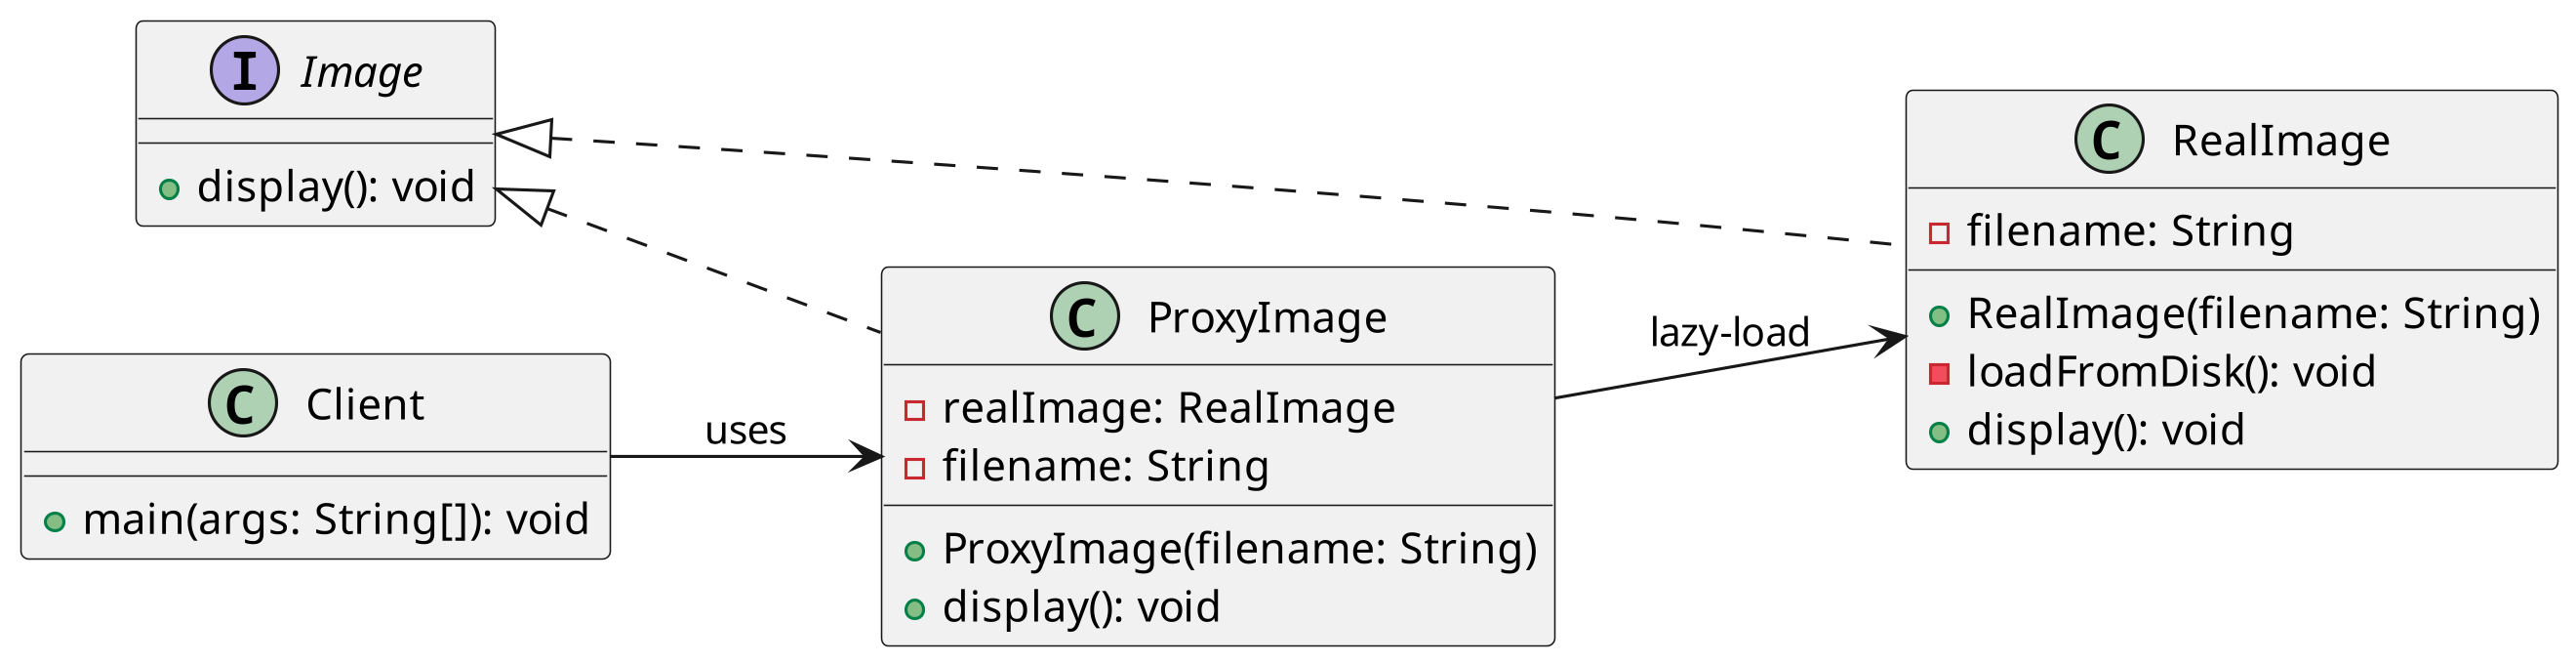
\includegraphics[width=\textwidth]{../figures/out/proxy.png}
	\caption{Struktur Pola Proxy}
	\label{fig:proxy}
\end{figure}

Contoh berikut menunjukkan penerapan pola Proxy pada sistem pengunduhan gambar (Gambar \ref{fig:proxy}), di mana gambar yang sebenarnya baru dimuat dari disk ketika benar-benar dibutuhkan (\textit{virtual proxy}).

\begin{lstlisting}[style=JavaStyle, caption={Subject: Image}, label={lst:proxy-subject}]
	public interface Image {
		void display();
	}
\end{lstlisting}

\begin{lstlisting}[style=JavaStyle, caption={RealSubject: RealImage}, label={lst:proxy-real}]
	public class RealImage implements Image {
		private String filename;
		
		public RealImage(String filename) {
			this.filename = filename;
			loadFromDisk();
		}
		
		private void loadFromDisk() {
			System.out.println("Loading " + filename);
		}
		
		@Override
		public void display() {
			System.out.println("Displaying " + filename);
		}
	}
\end{lstlisting}

\begin{lstlisting}[style=JavaStyle, caption={Proxy: ProxyImage}, label={lst:proxy-proxy}]
	public class ProxyImage implements Image {
		private RealImage realImage;
		private String filename;
		
		public ProxyImage(String filename) {
			this.filename = filename;
		}
		
		@Override
		public void display() {
			if (realImage == null) {
				realImage = new RealImage(filename); // Lazy instantiation
			}
			realImage.display();
		}
	}
\end{lstlisting}

\begin{lstlisting}[style=JavaStyle, caption={Client: Main}, label={lst:proxy-client}]
	public class Main {
		public static void main(String[] args) {
			Image image = new ProxyImage("photo.jpg");
			
			// Gambar belum dimuat
			System.out.println("Proxy created.");
			
			// Gambar dimuat dan ditampilkan saat pertama kali digunakan
			image.display();
			
			// Gambar tidak dimuat ulang
			image.display();
		}
	}
\end{lstlisting}

Penjelasan:
\begin{itemize}
	\item Antarmuka \texttt{Image} bertindak sebagai kontrak yang digunakan oleh klien.
	\item \texttt{RealImage} adalah kelas yang melakukan operasi aktual seperti memuat dan menampilkan gambar.
	\item \texttt{ProxyImage} menunda inisialisasi \texttt{RealImage} hingga benar-benar dibutuhkan (\textit{lazy loading}).
	\item Klien menggunakan \texttt{ProxyImage} seolah-olah ia berinteraksi langsung dengan \texttt{RealImage}.
\end{itemize}

Pola ini sangat berguna untuk mengelola objek yang mahal secara performa atau membutuhkan kontrol akses tambahan. Dengan pendekatan ini, pengembang dapat menyisipkan logika tambahan tanpa memodifikasi kelas inti (\texttt{RealImage}).


\section{Flyweight}

\subsection{Tujuan dan Konteks Penggunaan}

Pola \textit{Flyweight} merupakan salah satu pola struktural yang bertujuan untuk mengurangi konsumsi memori dan meningkatkan efisiensi performa dengan cara berbagi (sharing) objek-objek yang memiliki status serupa atau identik. Alih-alih membuat objek baru untuk setiap permintaan, pola ini memungkinkan beberapa klien menggunakan instansi objek yang sama secara bersamaan, selama bagian dari status objek tersebut tidak berubah (bersifat immutable atau \textit{intrinsic}).

Flyweight sangat berguna ketika aplikasi perlu menangani jumlah objek yang sangat besar namun dengan karakteristik internal yang sama. Dengan menyimpan hanya satu representasi dari objek dan menggunakan kembali representasi tersebut, pola ini secara signifikan mengurangi beban memori dan mempercepat proses instansiasi.

Pola ini memisahkan status objek menjadi dua bagian utama:
\begin{itemize}
	\item \textbf{Intrinsic State:} Informasi yang dapat dibagikan oleh banyak objek dan tidak berubah—misalnya bentuk huruf, warna, jenis bangunan.
	\item \textbf{Extrinsic State:} Informasi yang unik untuk tiap konteks penggunaan—misalnya posisi, ukuran, atau konteks runtime lainnya yang harus disediakan oleh klien.
\end{itemize}

Pola Flyweight sangat cocok digunakan ketika:
\begin{itemize}
	\item Aplikasi menciptakan jutaan objek dengan struktur atau nilai properti yang sama.
	\item Dibutuhkan penghematan memori dalam representasi objek skala besar, seperti tampilan teks, grafis, partikel dalam game, atau struktur data peta.
	\item Banyak objek yang dapat dibagikan (shared) tanpa efek samping atau konflik data antar pengguna.
\end{itemize}

Contoh umum penerapan Flyweight adalah dalam rendering teks di layar, di mana setiap huruf (misalnya karakter ‘a’) tidak perlu disimpan sebagai objek terpisah untuk setiap kemunculannya. Sebagai gantinya, satu objek huruf ‘a’ digunakan berulang kali untuk menampilkan huruf tersebut di berbagai posisi dalam dokumen atau antarmuka pengguna, dengan posisi dan gaya (warna, ukuran) sebagai status eksternal yang diberikan oleh klien.

Dengan pola ini, kita dapat mencapai efisiensi tinggi dalam penggunaan sumber daya, terutama dalam sistem dengan jumlah instansi objek yang besar dan bersifat homogen.

\subsection{Contoh Kasus Penggunaan}

Pola \textit{Flyweight} sering ditemukan dalam sistem yang membutuhkan efisiensi memori tinggi karena melibatkan jumlah objek yang sangat besar dan sering kali memiliki struktur atau data internal yang serupa. Berikut beberapa contoh kasus penggunaan nyata dari pola ini:

\textbf{1. Rendering Dokumen atau Teks Panjang}

Dalam sistem pengolahan dokumen seperti editor teks, browser, atau sistem layout buku digital, setiap karakter (huruf, angka, simbol) muncul berkali-kali. Alih-alih membuat objek baru untuk setiap karakter, sistem menggunakan pola Flyweight dengan satu objek per jenis karakter (\texttt{Character}), dan posisi serta gaya teks (ukuran, warna, posisi X/Y) diberikan secara eksternal saat rendering.

\textbf{2. Sistem Game: Partikel dan Objek Grafis}

Dalam game yang menampilkan banyak entitas identik seperti peluru, efek partikel, atau musuh dengan karakteristik serupa, pola Flyweight digunakan untuk menghemat memori. Misalnya, semua peluru memiliki sprite dan animasi yang sama, sehingga objek Flyweight untuk peluru dibagi ke banyak instance di berbagai posisi.

\textbf{3. Visualisasi Peta dan GIS (Geographic Information System)}

Ketika menampilkan ribuan landmark seperti pohon, gedung, atau simbol lalu lintas di peta digital, pola Flyweight dapat digunakan untuk merepresentasikan elemen-elemen ini hanya dengan satu objek per jenis. Data seperti lokasi geografis dan ukuran diberikan sebagai status eksternal, sementara bentuk dan simbol disimpan dalam objek flyweight.

\textbf{4. Representasi Simbol dalam Editor Grafik}

Dalam software desain seperti diagram editor atau CAD, objek seperti garis panah, node, dan label teks sering digunakan berulang. Dengan Flyweight, sistem hanya menyimpan satu instansi bentuk (misalnya satu jenis panah), dan menggunakannya berulang dengan posisi dan rotasi yang bervariasi.

\textbf{5. Sistem Simulasi dan Agen Massal}

Dalam simulasi yang menampilkan ribuan agen (seperti kendaraan, orang, atau robot), jika banyak agen memiliki perilaku atau tampilan serupa, Flyweight digunakan untuk mengelola karakteristik tetap (model 3D, animasi dasar), sementara informasi unik seperti kecepatan atau tujuan disimpan di luar objek flyweight.

\textbf{6. Cache Objek atau Pooling String}

Di Java, literal string secara default menggunakan pola Flyweight melalui \texttt{String Pool}. Dua variabel yang menyimpan string literal yang sama menunjuk ke objek yang sama di dalam pool untuk menghemat memori dan mempercepat pembandingan string.

Pola Flyweight dapat diterapkan secara eksplisit oleh pengembang, atau muncul secara implisit melalui optimasi sistem atau framework. Dalam semua kasus, tujuannya adalah menghindari redundansi dalam representasi objek yang identik dan meningkatkan performa dengan membagikan sumber daya secara efisien.

\subsection{Kelebihan dan Kekurangan}

Pola \textit{Flyweight} menawarkan efisiensi memori yang signifikan dalam sistem yang menangani sejumlah besar objek serupa. Namun, penggunaannya juga menimbulkan tantangan tertentu, terutama dalam hal manajemen status dan kompleksitas implementasi. Berikut adalah ringkasan kelebihan dan kekurangannya:

\textbf{Kelebihan:}
\begin{itemize}
	\item \textbf{Penghematan Memori:} Flyweight menghindari duplikasi data dengan membagikan objek yang identik. Hal ini sangat bermanfaat dalam sistem dengan jutaan instance, seperti rendering karakter dalam dokumen atau partikel dalam game.
	
	\item \textbf{Peningkatan Kinerja:} Dengan mengurangi beban alokasi dan garbage collection dari banyak objek identik, performa sistem dapat meningkat terutama dalam sistem grafis atau real-time.
	
	\item \textbf{Pemisahan State Ekstrinsik dan Intrinsik:} Pola ini mendorong desain yang lebih terstruktur dengan memisahkan data yang bisa dibagi (intrinsik) dan data unik (ekstrinsik) ke objek eksternal.
	
	\item \textbf{Dukungan untuk Struktur Tak Terbatas:} Dalam visualisasi atau simulasi skala besar, jumlah elemen yang dapat dimuat dalam memori menjadi lebih besar karena satu representasi dapat digunakan ulang.
	
	\item \textbf{Sering Didukung oleh Bahasa dan Framework:} Contoh seperti \texttt{String Pool} di Java dan \texttt{Font Glyph Cache} di sistem grafis adalah penerapan Flyweight secara otomatis oleh sistem.
\end{itemize}

\textbf{Kekurangan:}
\begin{itemize}
	\item \textbf{Manajemen State Lebih Rumit:} Karena data ekstrinsik dikelola secara eksternal, pengembang harus memastikan status unik diberikan secara konsisten kepada objek flyweight saat digunakan.
	
	\item \textbf{Kompleksitas Desain:} Struktur kode bisa menjadi lebih kompleks karena perlu membedakan antara data yang bisa dibagi dan tidak bisa dibagi, serta mengelola cache atau registry flyweight.
	
	\item \textbf{Tidak Cocok untuk Objek dengan State yang Sangat Variatif:} Jika objek memiliki banyak atribut unik atau sering berubah-ubah, manfaat flyweight akan menurun dan mungkin justru memperumit desain.
	
	\item \textbf{Resiko Masalah Thread-Safety:} Ketika objek flyweight digunakan secara bersamaan di berbagai thread, sinkronisasi diperlukan pada data ekstrinsik untuk mencegah konflik.
	
	\item \textbf{Kesulitan Debugging dan Tracking:} Karena objek yang sama digunakan di banyak tempat, melacak perilaku spesifik atau kesalahan bisa lebih sulit terutama saat state tidak tersimpan dalam objek itu sendiri.
\end{itemize}

Secara keseluruhan, pola \textit{Flyweight} ideal untuk sistem dengan skala besar dan struktur objek yang sering berulang, namun perlu implementasi yang hati-hati agar tidak menimbulkan kompleksitas dan bug tersembunyi.


\subsection{Implementasi dalam Java}

Implementasi pola \textit{Flyweight} dalam Java berfokus pada pemisahan state intrinsik (yang dapat dibagi) dan state ekstrinsik (yang unik untuk setiap penggunaan). Objek-objek flyweight biasanya dibuat dan dikelola oleh suatu \texttt{FlyweightFactory} yang bertanggung jawab untuk menyimpan dan mengembalikan instance yang sudah ada jika tersedia, atau membuat instance baru jika belum ada.

\begin{figure}[h]
	\centering
	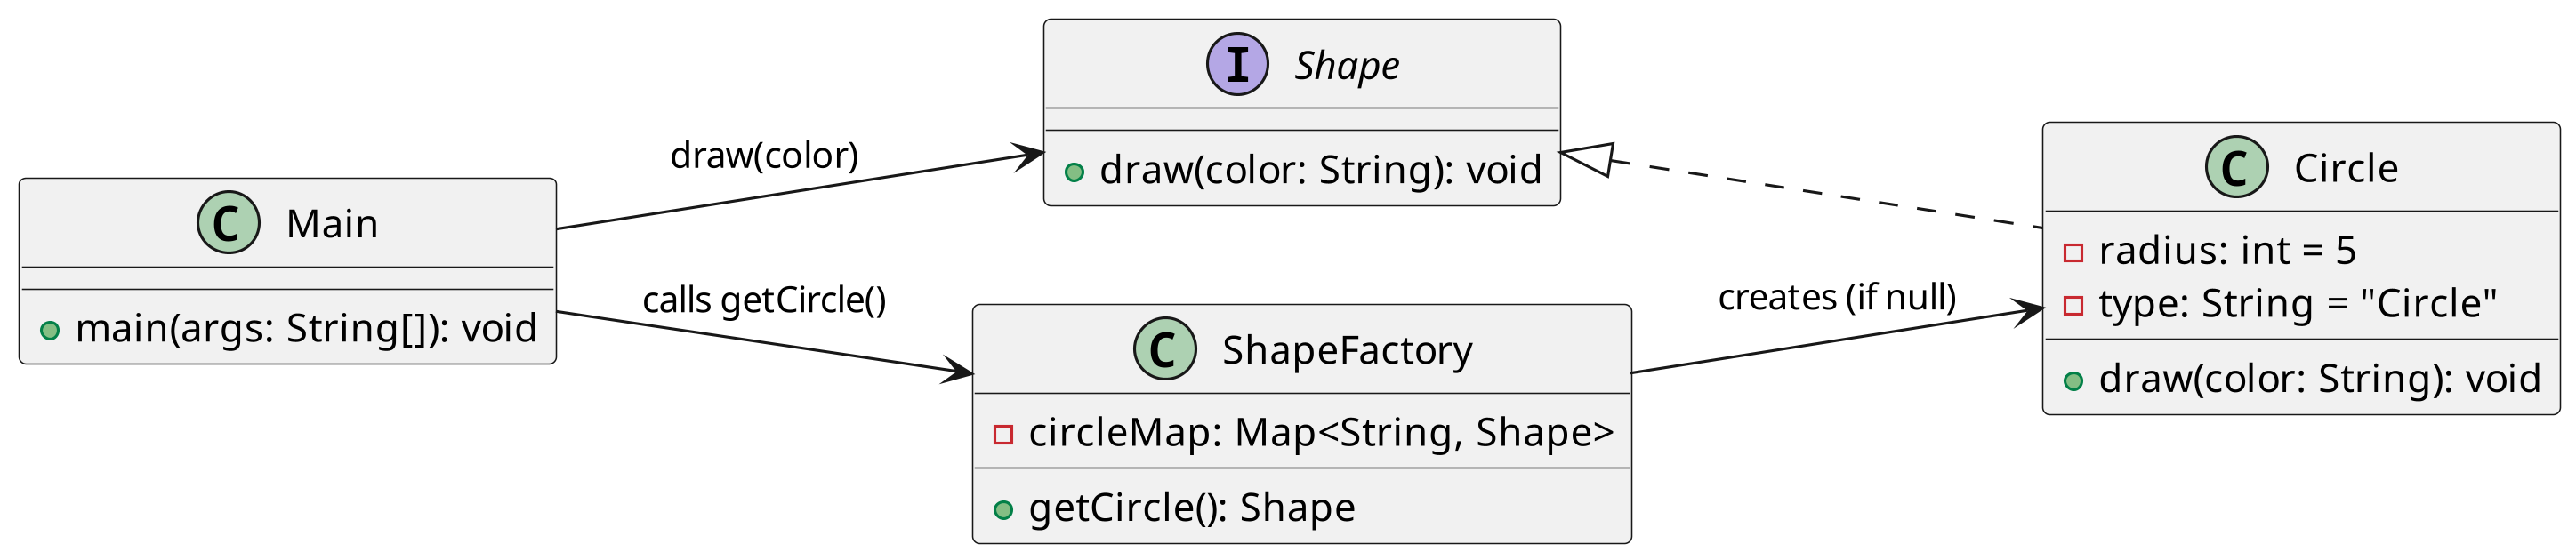
\includegraphics[width=\textwidth]{../figures/out/flyweight.png}
	\caption{Struktur Pola Flyweight}
	\label{fig:flyweight}
\end{figure}

Pola ini sangat cocok diterapkan dalam sistem yang memiliki banyak objek identik (Gambar \ref{fig:flyweight}), seperti karakter dalam editor teks, pohon-pohon dalam permainan, atau titik koordinat dalam grafik besar.

Berikut adalah struktur dasar implementasi pola Flyweight dalam Java:

\begin{lstlisting}[style=JavaStyle, caption={Flyweight: Shape}, label={lst:flyweight-shape}]
	public interface Shape {
		void draw(String color); // color = ekstrinsik
	}
\end{lstlisting}

\begin{lstlisting}[style=JavaStyle, caption={Flyweight Konkret: Circle}, label={lst:flyweight-circle}]
	public class Circle implements Shape {
		private final int radius = 5; // state intrinsik
		private final String type = "Circle"; // state intrinsik
		
		@Override
		public void draw(String color) {
			System.out.println("Drawing " + type + " with radius " + radius + " and color " + color);
		}
	}
\end{lstlisting}

\begin{lstlisting}[style=JavaStyle, caption={Flyweight Factory: ShapeFactory}, label={lst:flyweight-factory}]
	import java.util.HashMap;
	import java.util.Map;
	
	public class ShapeFactory {
		private static final Map<String, Shape> circleMap = new HashMap<>();
		
		public static Shape getCircle() {
			Shape circle = circleMap.get("circle");
			if (circle == null) {
				circle = new Circle();
				circleMap.put("circle", circle);
				System.out.println("Creating new Circle instance.");
			}
			return circle;
		}
	}
\end{lstlisting}

\begin{lstlisting}[style=JavaStyle, caption={Client: Menggunakan Flyweight}, label={lst:flyweight-main}]
	public class Main {
		public static void main(String[] args) {
			String[] colors = { "Red", "Green", "Blue", "Yellow" };
			
			for (int i = 0; i < 10; i++) {
				Shape circle = ShapeFactory.getCircle();
				circle.draw(colors[i % colors.length]); // ekstrinsik
			}
		}
	}
\end{lstlisting}

Penjelasan dari contoh di atas:
\begin{itemize}
	\item \texttt{Shape} adalah antarmuka flyweight yang hanya mendefinisikan metode umum (\texttt{draw()}), dengan parameter eksternal sebagai state ekstrinsik.
	\item \texttt{Circle} menyimpan state intrinsik seperti \texttt{radius} dan \texttt{type}, yang sama untuk semua instance lingkaran.
	\item \texttt{ShapeFactory} menggunakan cache berbasis \texttt{Map} untuk menyimpan objek \texttt{Circle} agar dapat digunakan ulang.
	\item \texttt{Main} menunjukkan bahwa meskipun objek \texttt{Circle} hanya dibuat sekali, ia bisa digunakan dengan warna berbeda (state ekstrinsik).
\end{itemize}

Pendekatan ini sangat efisien dalam sistem berskala besar, karena menghindari penciptaan objek berulang dengan data yang sama dan mengurangi beban pada garbage collector.




\section{Kesimpulan}

Bab ini telah membahas lima pola struktural lanjutan yang memainkan peran penting dalam meningkatkan modularitas, efisiensi, dan skalabilitas sistem perangkat lunak. Pola \textit{Facade} menyederhanakan interaksi dengan subsistem kompleks melalui antarmuka tunggal, sementara \textit{Proxy} memberikan kendali tambahan terhadap objek asli dengan memperantarai aksesnya. \textit{Flyweight} memungkinkan penghematan memori melalui penggunaan objek bersama dalam skenario berskala besar.

Dengan memahami dan menerapkan pola-pola ini secara tepat, pengembang dapat merancang sistem yang lebih bersih, lebih mudah dipelihara, dan lebih tangguh terhadap perubahan. Masing-masing pola memiliki kekuatan yang khas dan penerapannya perlu disesuaikan dengan kebutuhan desain serta karakteristik domain aplikasi. Penguasaan pola struktural ini menjadi fondasi penting dalam menciptakan perangkat lunak yang berorientasi objek dan scalable di berbagai konteks pengembangan modern.

